\section{Additional Mechanics}

\subsection{HUD}

\begin{figure}[H]
	\centering
	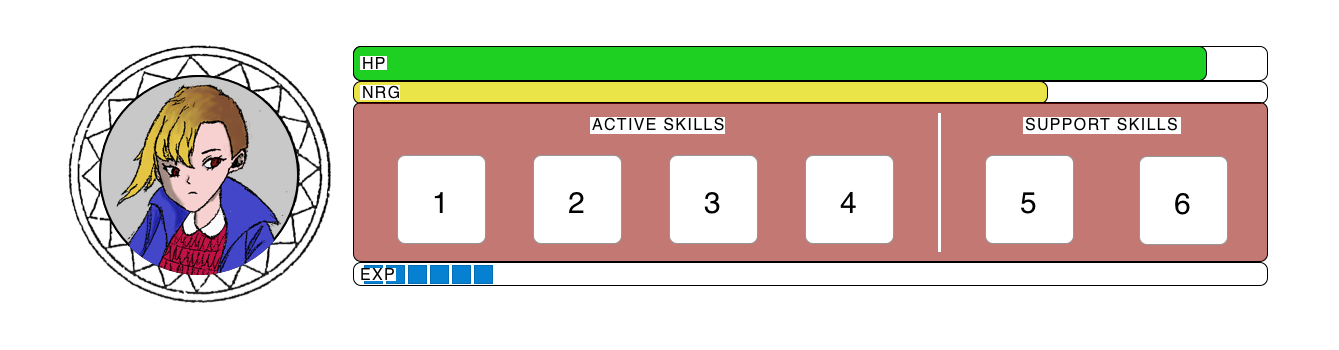
\includegraphics[width=14cm]{images/hud/HUD_life_green.png}
\end{figure}

Alongside Elby's health bar (the green one in the picture above), players will see in the HUD also the energy bar (the yellow one in the picture). “Energy” represent the amount of Elby’s telekynesis power, and it decreases when she uses her prowness to perform an active skill (see paragraph x).\\\\
A unique mechanic of this game is applied when Elby runs out of energy. The player is still allowed to make use of the active abilities drawing on the character's HP bar instead of using energy.\\
This double-edged sword allows the player to extend combat and exploration, but makes him vulnerable to fatal monster attacks.
Therefore energy is essential for survival and for this reason we have decided to add an auto-recovery that allows the latter to regenerate over time, specifically 1 NRG/turn.



\begin{figure}[H]
	\centering
	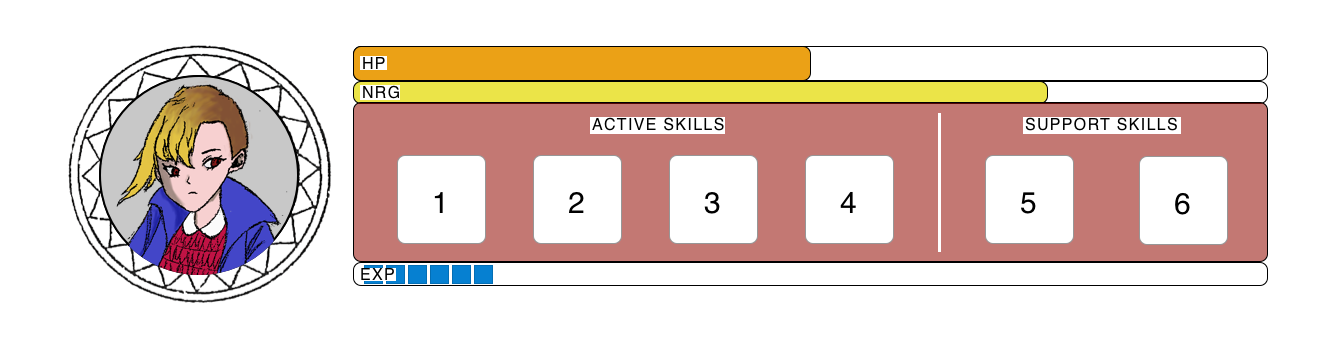
\includegraphics[width=14cm]{images/hud/HUD_life_orange.png}
	\caption*{HP > 25\% and HP $\leq$ 50\%}
\end{figure}

\begin{figure}[H]
	\centering
	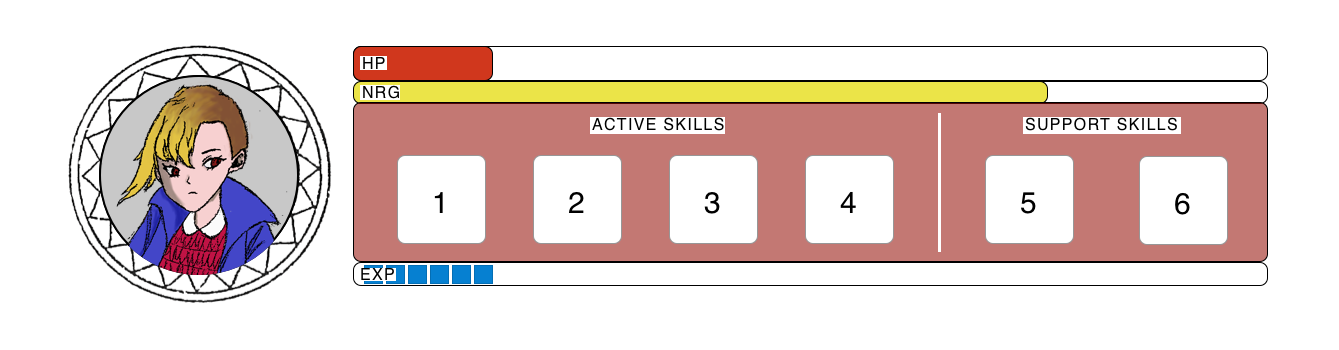
\includegraphics[width=14cm]{images/hud/HUD_life_red.png}
	\caption*{HP $\leq$ 25\%}
\end{figure}

The picture of Elby inside the circle of the HUD changes accordingly to the status of the energy bar. Her facial expression changes when she is in combat and her energy has dropped under 20\%. In this case the figure will show blood dripping from the nose and will remain so until the fight is finished and the energy restored. For example, in the image above, Elby maintains the standard avatar although her life has fallen below 20\% (in this specific case the edge of the game screen will start to flash red).

\subsection{Skills and Items}
During the adventure, the player will unlock several Elby abilities, called Active Skills. These skills can be assigned as the player wishes in the 4 slots available in the Active Skills section of the HUD and can be changed everytime Elby visits a checkpoint. We made this choice because we wanted to allow the player to create a personalized set.\\\\
Sometimes elby will meet characters who decide to follow her on the journey. These NPCs have unique abilities, called Support Skills, which will be displayed in the Support Skills section of the HUD and they can not be changed. Every Support Skill will be explained below.\\\\
Items can be also be set in the Active Skills's HUD section, letting the player decide whether to use multiple skills with few objects or vice versa.\\\\
Being that a turn corresponds to 3 seconds, both Active and Support Skills provide a multiple cooldown of 3 based on the skill damage and effect.

\subsection{Items and crafting}

\subsubsection{Consumable items}

\subsubsection{Initial inventory prediction}
The potential inventory of the player at the beginning of the level could be:
\begin{itemize}
	\item Coal x2
	\item Fresh root x2
	\item Demorat tail x1
	\item Stick x3
	\item Bracelet x1
	\item Small potion x1
	\item Energy potion x1
	\item Bag x1
	\item Rock x3
	\item Demodog meat x2
	\item Sand x1
\end{itemize}

\subsubsection{Collectible items}

\newpage

\subsection{Checkpoints and Game Saves}

\begin{figure}[H]
	\centering
	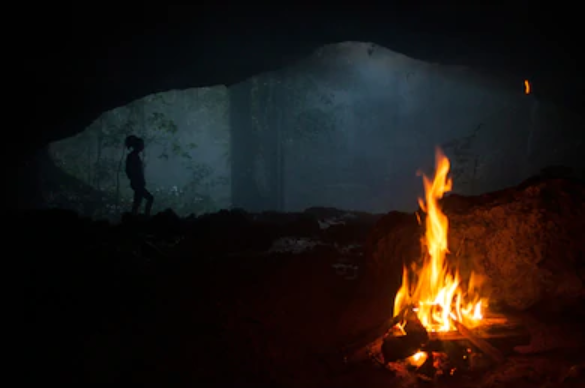
\includegraphics[width=14cm]{images/visual_ref/checkpoint.png}
\end{figure}

Scattered around the levels players can find safe places to take refuge and light a bonfire. These spots act as checkpoints.\\
In the Giant Chasm there are 3 of them, located in the Cerberus room (activated only after defeating the miniboss), at the beginning of the second section of the level and in the middle of the third section.\\
While Elby is at the bonfire, she can cook food, craft items, change her active skills and rest, fully recovering both hit points and mana points, allowing however the respawn of all the monsters in the section (only if they have been previously defeated).\\
We have decided not to allow the player to use quick travel between the various checkpoints on the map to remain consistent with the theme of the game (the player can still use it to move between the game areas). We also thought that the best solution for saving the game is an auto-save every time the player visits a bonfire. This allows us to predict the player's actions and movements with more precision, incentivize him to plan a strategy to cross the maps and prevent him from passing certain key points of the level simply by saving and repeating, consequently increasing the difficulty and the overall challenge.


